\section{Einleitung}

\begin{itemize}
  \item \underline{Anwendungsfälle:}
  \begin{enumerate}
    \item Aus einer Menge von Graphen soll eine Funktion für Klassifizierungs- oder Regressionsprobleme gelernt werden, die auf nicht bekannte Graphen angewendet werden kann
    \item lerne Graph-Repräsentationen, um auf Graph-Eigenschaften (fehlende Kanten, Knoteneigenschaften) unbekannter Graphen zu schließen
  \end{enumerate}
\item \underline{Graphrepräsentation:}
  \begin{itemize}
    \item Graphen können gerichtet oder ungerichtet sein
    \item Graphen können zyklisch sein
    \item Graphen können mehrere unterschiedliche Kantentypen besitzen (mehrere Perceptive-Field-Layer)
    \item Graphen können mehrere diskrete oder kontinuierliche Werte an ihren Knoten haben
  \end{itemize}
\item Methode berechnet lokal verbundene Nachbarschaften der Graphen und benutzt sie als die \emph{Receptive Fields} des CNN
\item die Methode kann für Graphen mit gewichteten Kanten erweitert werden
\end{itemize}

\begin{figure}[h]
  \centering
  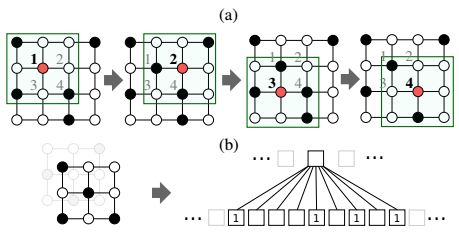
\includegraphics[width=.5\textwidth]{images/cnn_graph}
\end{figure}

\begin{itemize}
  \item \underline{Idee:} repräsentiere Bilder als Graph
    \begin{itemize}
      \item ein Bild kann als Graph repräsentiert werden, indem die Knoten jeweils einen Pixel repräsentieren und es eine Kante zwischen zwei Knoten gibt, wenn deren Pixel benachbart sind
      \item die lokale Nachbarschaft eines Pixels wird repräsentiert als ein Quadrat um den Punkt (hier $3 \times 3$)
      \item Aus der Nachbarschaft kann ein Merkmal ermittelt werden
    \end{itemize}
  \item üblicherweise gibt es keine räumliche Anordnung einer Graph-Repräsentation
  \item \underline{Probleme:}
    \begin{enumerate}
      \item Welche Nachbarschaften um welche Knoten und in welcher Reihenfolge bilden die Receptive Fields?
      \item Wie können die einzelnen Nachbarschafts-Graphen in einem Vektor repräsentiert werden (Normalisierung)?
    \end{enumerate}
  \item \underline{Verfahren:}
    \begin{enumerate}
      \item bestimme eine Knoten-Auswahl inklusive Reihenfolge
      \item bestimme den Nachbarschafts-Graphen um diesen Knoten mit genau $k$ Knoten
      \item normalisiere die Nachbarschafts-Graphen
      \item füttere sie in ein CNN
    \end{enumerate}
\end{itemize}
